\documentclass[11pt, a4]{article}

\usepackage{graphicx}
\usepackage{subfig}
\usepackage{float}
\usepackage{amsmath}

\newcommand{\norm}[1]{\left\lVert#1\right\rVert}

\begin{document}
Daniel Braithwaite \\
300313770

\section{Question 1 - Lena}
\subsection{Approximations}
Approximations with rank 10, 20, 50, 100, 200, 400
\begin{figure}[H]
	\centering
	\subfloat[r = 10]{{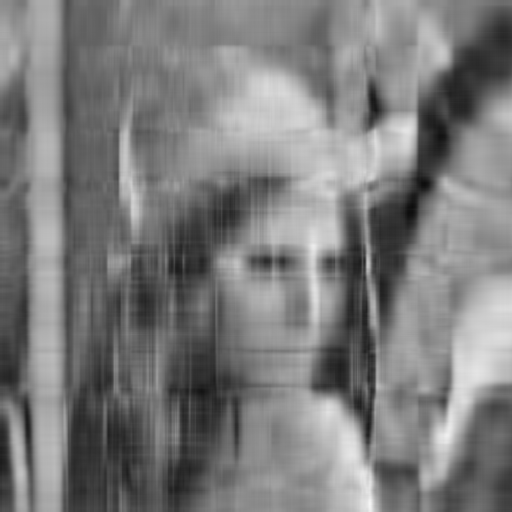
\includegraphics[width=3cm]{images/Julia_Rank10} }}%
	\qquad
	\subfloat[r = 20]{{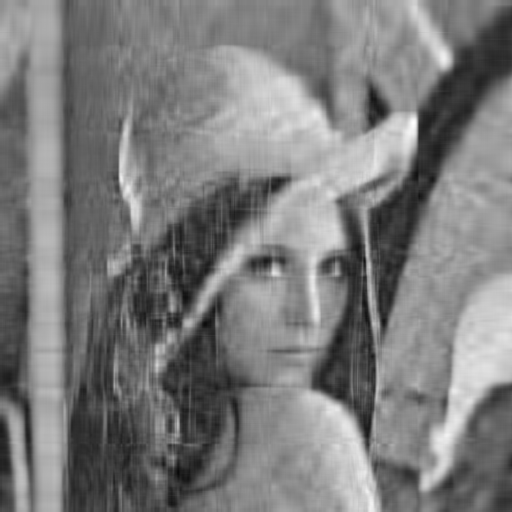
\includegraphics[width=3cm]{images/Julia_Rank20} }}%
	\qquad
	\subfloat[r = 50]{{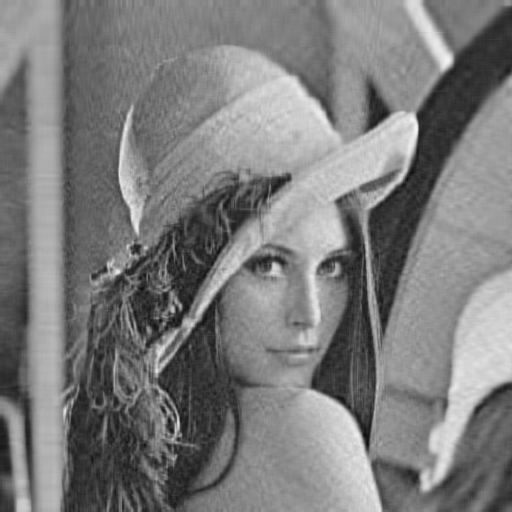
\includegraphics[width=3cm]{images/Julia_Rank50} }}%
\end{figure}

\begin{figure}[H]
	\centering
	\subfloat[r = 100]{{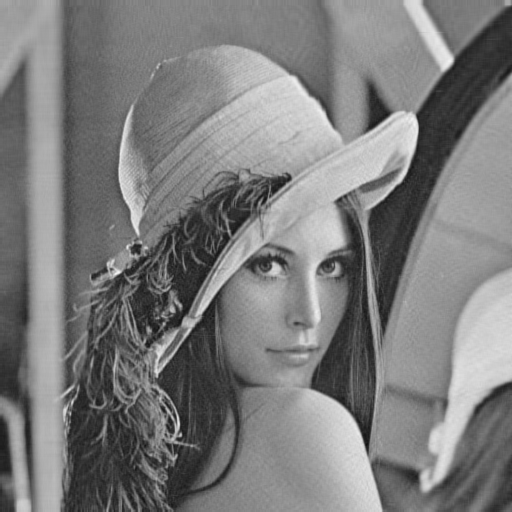
\includegraphics[width=3cm]{images/Julia_Rank100} }}%
	\qquad
	\subfloat[r = 200]{{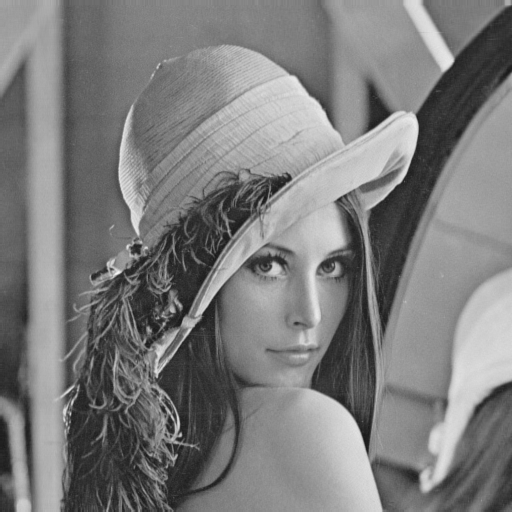
\includegraphics[width=3cm]{images/Julia_Rank200} }}%
	\qquad
	\subfloat[r = 400]{{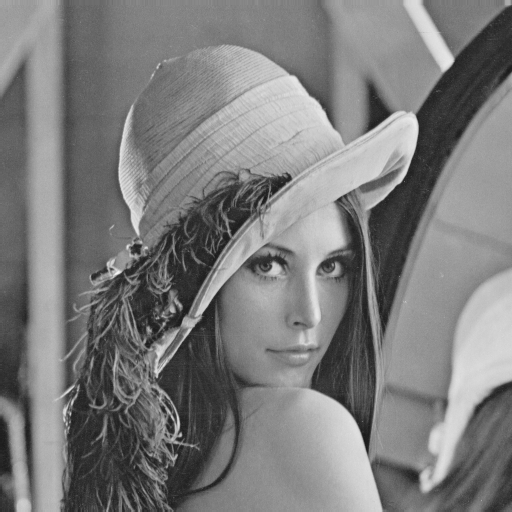
\includegraphics[width=3cm]{images/Julia_Rank400} }}%
\end{figure}

\subsection{Error Discussion}
From inspection of the program output we can see that the error computed using the \textbf{frobenius} norm is equal to the square root of the sum of eigen values that are zeroed out to achive the approximation. We see this is true from the folowing. We have $A = U \Sigma V^{T}$ by SVD, and then we get the rank $k$ approximation of k as $\widetilde{A} = U \widetilde{\Sigma} V^{T}$. Now considerthe folowing

\begin{equation}
\begin{aligned}
	A - \widetilde{A} &= U \Sigma V^{T} - U \widetilde{\Sigma} V^{T} \\&= U (\Sigma - \widetilde{\Sigma}) V^{T} \\&= U \Sigma^\prime V^{T}
\end{aligned}
\end{equation}
\\
Where the diagonal of $\Sigma^\prime$ contains all singular values not in $\widetilde{\Sigma}$.\\

So finally $\norm{A - \widetilde{A}}_{Fro} = \sqrt{\sum_{i=k+1} (\sigma_i^\prime)^2}$ \\
As we saw experementally


\section{Question 2 - Yalefaces}
\subsection{Approximations}
Approximations with rank 10, 20, 40, 80, 120
\begin{figure}[H]
	\centering
	\subfloat[r = 10]{{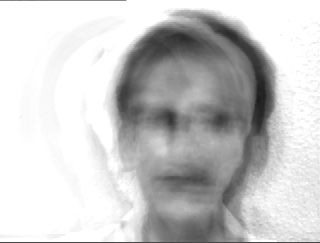
\includegraphics[width=1.5cm]{images/Image-5-10} }}%
	\qquad
	\subfloat[r = 20]{{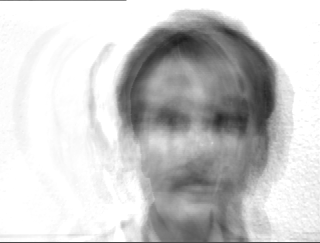
\includegraphics[width=1.5cm]{images/Image-5-20} }}%
	\qquad
	\subfloat[r = 40]{{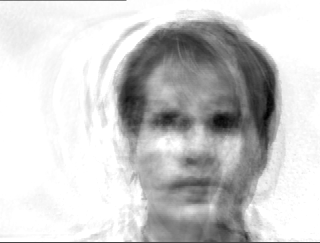
\includegraphics[width=1.5cm]{images/Image-5-40} }}%
	\qquad
	\subfloat[r = 80]{{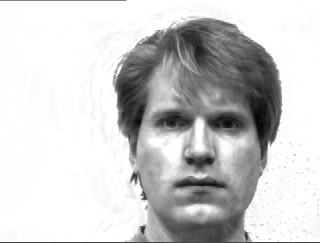
\includegraphics[width=1.5cm]{images/Image-5-80} }}%
	\qquad
	\subfloat[r = 120]{{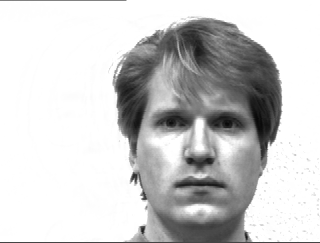
\includegraphics[width=1.5cm]{images/Image-5-120} }}%
	\caption{Image 5}
\end{figure}

\begin{figure}[H]
	\centering
	\subfloat[r = 10]{{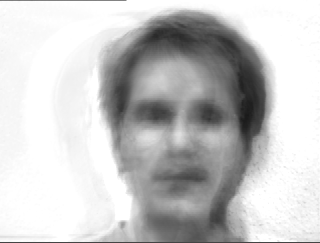
\includegraphics[width=1.5cm]{images/Image-10-10} }}%
	\qquad
	\subfloat[r = 20]{{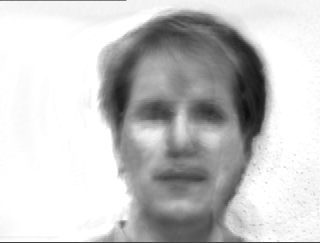
\includegraphics[width=1.5cm]{images/Image-10-20} }}%
	\qquad
	\subfloat[r = 40]{{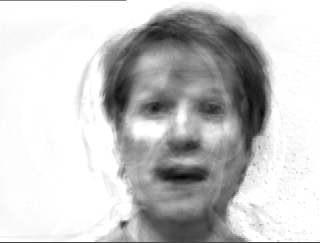
\includegraphics[width=1.5cm]{images/Image-10-40} }}%
	\qquad
	\subfloat[r = 80]{{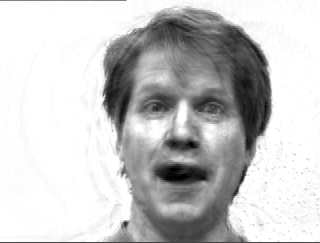
\includegraphics[width=1.5cm]{images/Image-10-80} }}%
	\qquad
	\subfloat[r = 120]{{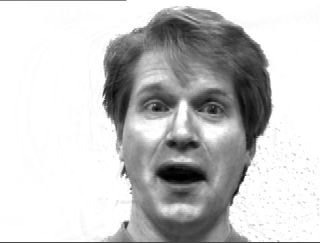
\includegraphics[width=1.5cm]{images/Image-10-120} }}%
	\caption{Image 10}
\end{figure}

\begin{figure}[H]
	\centering
	\subfloat[r = 10]{{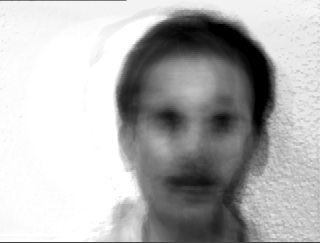
\includegraphics[width=1.5cm]{images/Image-14-10} }}%
	\qquad
	\subfloat[r = 20]{{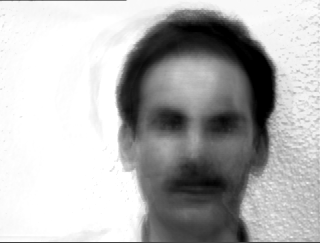
\includegraphics[width=1.5cm]{images/Image-14-20} }}%
	\qquad
	\subfloat[r = 40]{{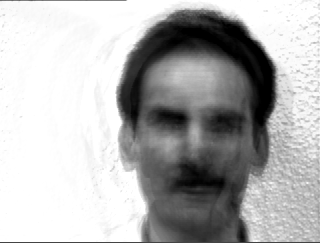
\includegraphics[width=1.5cm]{images/Image-14-40} }}%
	\qquad
	\subfloat[r = 80]{{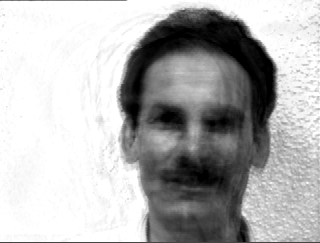
\includegraphics[width=1.5cm]{images/Image-14-80} }}%
	\qquad
	\subfloat[r = 120]{{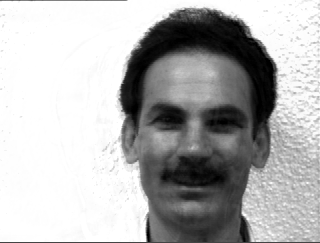
\includegraphics[width=1.5cm]{images/Image-14-120} }}%
	\caption{Image 14}
\end{figure}

\begin{figure}[H]
	\centering
	\subfloat[r = 10]{{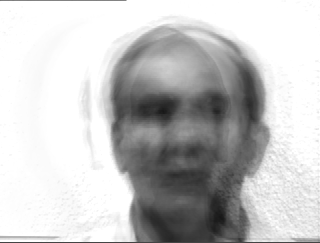
\includegraphics[width=1.5cm]{images/Image-50-10} }}%
	\qquad
	\subfloat[r = 20]{{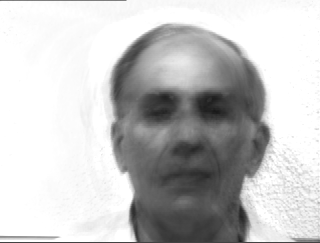
\includegraphics[width=1.5cm]{images/Image-50-20} }}%
	\qquad
	\subfloat[r = 40]{{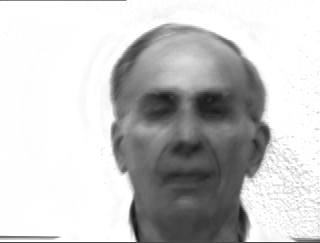
\includegraphics[width=1.5cm]{images/Image-50-40} }}%
	\qquad
	\subfloat[r = 80]{{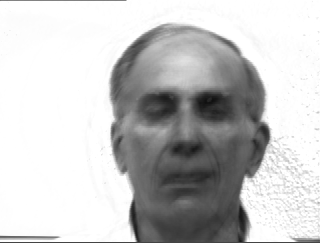
\includegraphics[width=1.5cm]{images/Image-50-80} }}%
	\qquad
	\subfloat[r = 120]{{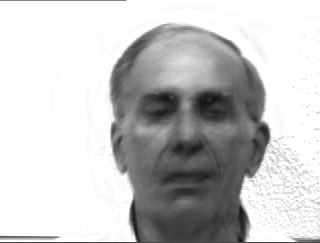
\includegraphics[width=1.5cm]{images/Image-50-120} }}%
	\caption{Image 50}
\end{figure}

\begin{figure}[H]
	\centering
	\subfloat[r = 10]{{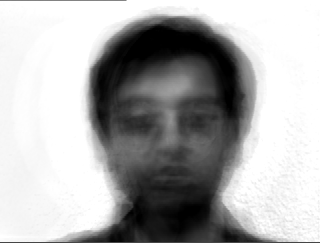
\includegraphics[width=1.5cm]{images/Image-67-10} }}%
	\qquad
	\subfloat[r = 20]{{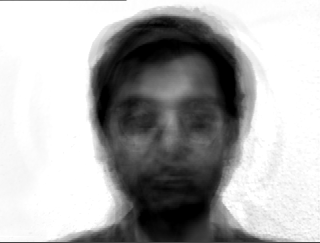
\includegraphics[width=1.5cm]{images/Image-67-20} }}%
	\qquad
	\subfloat[r = 40]{{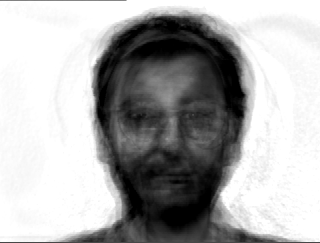
\includegraphics[width=1.5cm]{images/Image-67-40} }}%
	\qquad
	\subfloat[r = 80]{{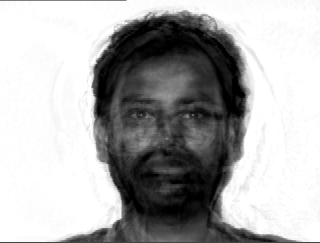
\includegraphics[width=1.5cm]{images/Image-67-80} }}%
	\qquad
	\subfloat[r = 120]{{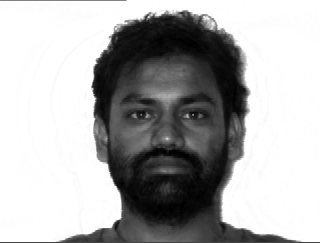
\includegraphics[width=1.5cm]{images/Image-67-120} }}%
	\caption{Image 67}
\end{figure}

\begin{figure}[H]
	\centering
	\subfloat[r = 10]{{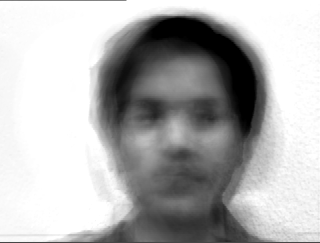
\includegraphics[width=1.5cm]{images/Image-100-10} }}%
	\qquad
	\subfloat[r = 20]{{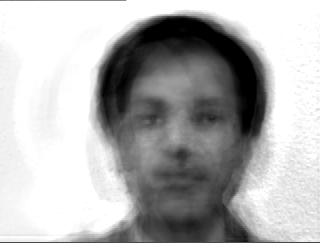
\includegraphics[width=1.5cm]{images/Image-100-20} }}%
	\qquad
	\subfloat[r = 40]{{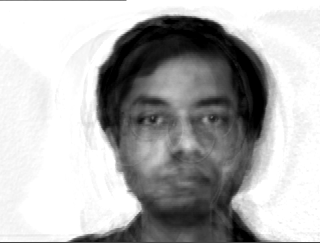
\includegraphics[width=1.5cm]{images/Image-100-40} }}%
	\qquad
	\subfloat[r = 80]{{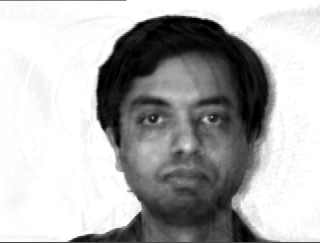
\includegraphics[width=1.5cm]{images/Image-100-80} }}%
	\qquad
	\subfloat[r = 120]{{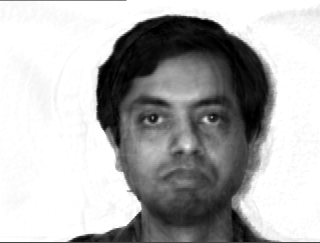
\includegraphics[width=1.5cm]{images/Image-100-120} }}%
	\caption{Image 100}
\end{figure}

\subsection{Error Discussion}
\textbf{See section 1.2}

\section{Question 3 - SVD - PCA Relationship}
Take X as our data matroix (we assume X has been mean centered). Then PCA is asking us to compute the eigenvalues and eigenvectors of the covariance matrix of X which is
$XX^T$. As $XX^T$ is symmetric by the spectral theorem we have $X = K A K^T$. Where A is diagonal with entries corosponding to the eigenvalues of $XX^T$ and K is orthonormal with columns corosponding to the eigenvectors of $XX^T$.\\

Now we consider the SVD of X, $X = U \Sigma V^T$, take $XX^T = (U \Sigma V^T)(U \Sigma V^T)^T = U \Sigma^2 U^T$. So the singular values of $X$ corospond to the square roots of the eigen values of $XX^T$

\end{document}